\chapter{N-propyl-cyclohexane (PCH) Model}
\section{Kinetic Model}

Liquid transportation fuels are continuously used in different applications and the necessity to understand the reactivity of those fuels has been explored extensively in Chapter 1. Now we turn to the actual oxidation of the second primary reference fuel (PRF) of this work, which is n-propyl-cyclohexane. N-propyl-cyclohexane is a member of the straight chain cycloalkane hydrocarbons commonly called naphthenes. Naphthenes are usually present in liquid transportation fuels adequate knowledge of their combustion properties is of great interest in the design of Homogeneous Charge Compression Ignition (HCCI) engines as alternatives to spark ignition (SI) engines. While this study has been applied to large and heavy duty machinery, naphthenes play an important role in the overall composition of liquid transportation fuels as well as the design and optimization of HCCI engines \cite{Aceves1999CompressionCombustion}. Although, alkanes both straight chain and branched chain alkanes dominate the composition of liquid transportation fuels with 80\% - 90\% being either n-decane, n-dodecane for straight chain reference fuel composition and iso-octane as a model fuel for branched alkanes , common naphthenes found in transportation fuels include cyclohexane, alkyl-cyclohexane from methyl-cyclohexane, ethyl-cyclohexane and up to n-butyl-cyclohexane \cite{Granata2003ANaphthenes}. 

The structure of n-propyl-cyclohexane looked at in this work is the straight chain propyl-cyclohexane in the skeletal structure of fig.\ref{fig:n-pch}. N-propyl-cyclohexane has the molecular formula of \ce{C_9H_18} since it is a member of the cycloalkane family with a general structural formula of \ce{C_nH_{2n}}. 

\begin{figure}[!htp]
    \centering
    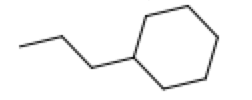
\includegraphics[scale=0.5, keepaspectratio]{images/pch-skeletal-formula.png}
    \caption{n-propyl-cyclohexane Structure}
    \label{fig:n-pch}
\end{figure}




N-propyl-cyclohexane has long been identified as a constituent compound in the representation of transportation fuels \cite{Pousse2010LeanN-Propylcyclohexane}. Since it is representative of the important compounds in transportation fuels, enormous work has been done on the auto-ignition characteristics of the fuel. Experimental investigation of n-propyl-cyclohexane includes ignition delay time measurements in shock tubes and rapid compression machines (RCM)  \cite{Dubois2009ExperimentalConditions}\cite{Crochet2010AConditions}\cite{Tian2014ComparativeN-Propylcyclohexane}, laminar flame speeds \cite{Pousse2010LeanN-Propylcyclohexane}\cite{Crochet2010AConditions}, chemical structure from pyrolysis and oxidation in pressure flow reactors and jet stirred reactors \cite{Bales-Gueret1992ExperimentalReactor} \cite{Ristori2001TheModeling}\cite{Dagaut2015TheStudy}\cite{Dagaut2014}\cite{Dagaut2016ExperimentalSurrogates}\cite{Gokulakrishnan2008IgnitionFuel}\cite{Gokulakrishnan2007ExperimentalConditions}. These experimental measurements provide a basis with which to compare chemical kinetic models of n-propyl-cyclohexane as means of validating the mechanisms. Similarly, several kinetic models of n-propyl-cyclohexane have been published over the years using the chemical kinetic mechanism generation code EXGAS \cite{Warth2000ComputerOxidation} used by Battin-Leclerc and others \cite{Battin-Leclerc2008DetailedSurrogates}, models have also been published on n-propyl-cyclohexane using the CHEMKIN suite code from Dubois et al \cite{Dubois2009ExperimentalConditions}, n-propyl-cyclohexane model has also been deduced based on surrogate modeling of jet fuels using a biokerosene fuel surrogate model of n-hexadecane, n-propylcyclohexane, n-propylbenzene and n-decane as described by Dagaut et al \cite{Dagaut2007ChemicalCombustion} as well as the synthetic diesel fuel surrogate model of Mati et al.\cite{Mati2007TheModeling} that consisted of n-hexadecane(36.1\% by weight, 23.5\% vol.), n-propylcyclohexane (23.1\% weight, 26.9\% vol.), n-propylbenzene (18.7\% weight, 22.9\% vol.), iso-octane(14.7\% weight, 19\% vol.) and 1-methylnaphthalene (7.4\% weight, 7.7\% vol.). Westbrook et al \cite{Westbrook2009AN-hexadecane} published a combined model of n-octane to n-hexadecane, Wang et al then constructed a very detailed model that integrates various fuels including n-alkane, cycloalkanes and alkyl-cycloalkanes in the JetSurF v2.0 model \cite{Wang2010A2.0}.Although, submechnanisms and skeletal models of n-propyl-cyclohexane have been built in the past by Ristori et al \cite{Ristori2001TheModeling}, more recently, Abbasi et al \cite{Abbasi2018KineticFormation} built a submechanism for n-propyl-cyclohexane coupled with new pathways for polycyclic aromatic hydrocarbons (PAH) formation. All these n-propyl-cyclo-hexane models built have been validated against various experimental conditions and there is still ongoing work to the determination of new pathways, reaction intermediates, better estimation of thermo-chemical parameters and rate constants for these kinetic models. \par
\vspace{0.5cm}
The n-propyl-cyclohexane model conditions as constructed in RMG have been outlined in Chapter 2 table \ref{tab:PRF_table1} as well as the reactor conditions used in table \ref{tab:PRF_table2} and table \ref{tab:PRF_table3}. This section is going to focus exclusively on the reaction pathways of n-propyl-cyclohexane, only the high-temperature reaction mechanism as well as the flux diagram of fig. \ref{fig:f2} of the RMG model validated against published experiments with comparison to other published n-propyl-cyclohexane kinetic models. The n-propyl-cyclohexane model constructed in RMG was done on the basis of seed mechanisms of 
Burke et al\cite{Burke2012ComprehensiveCombustion}, Hashemi et al\cite{Hashemi2016High-pressureMethane} and Li et al\cite{Li2017TheoreticalC2H4} in the exact order as shown. 

The reaction library used ``violator\textunderscore fixes\textunderscore 500-1500K'', was written on the basis of a previous propyl-cyclohexane RMG model that had significant collision limit violators. These violators represent rate coefficents higher than the collision limit from the Lennard-Jones potential and was indicated by Chen et al \cite{Chen2017ViolationModels}, that these rate coefficients especially for three-body reactions are much higher than the collision limit and thus are nonphysical. Using this definition, the rates both forward and reverse rate coefficients were compared against the collision limits set by the Lennard-Jones potential and the result was that the collision frequency of the Arrhenius rates were reduced by the factor above which it went above the collision limit as seen in the plot of fig. \ref{fig:pch-collision-limit}.


\begin{figure}[!h]
    \centering
    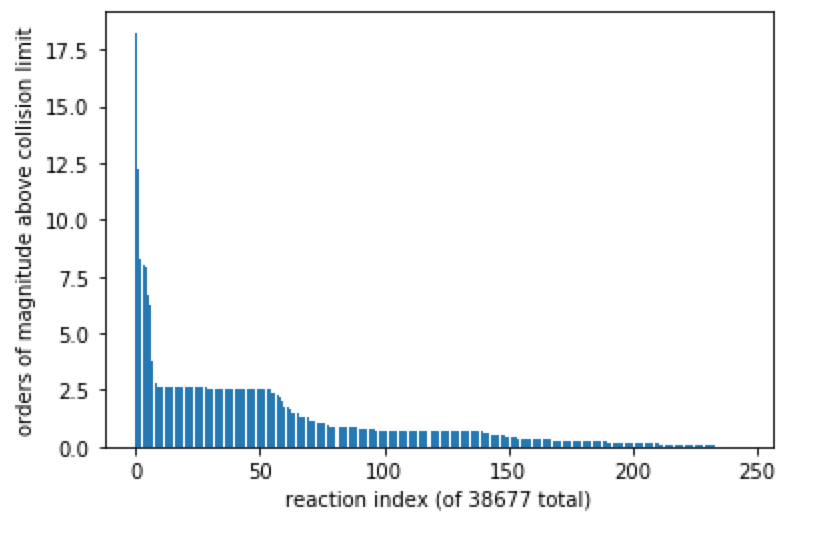
\includegraphics[scale=0.75, keepaspectratio]{images/pch-collision-violators.png}
    \caption{Collision rate violators of the initial RMG propyl-cyclohexane model based on the factor above the collision limit set by the Lennard-Jones Potential collision limit described in Wang et al. \cite{Wang2017Molecular-levelTemperature}}
    \label{fig:pch-collision-limit}
\end{figure}





The collision rate limit is defined below in equ.\ref{equ:collision limit} in RMG 
\begin{equation}
    k_{coll,i}(T)= \sqrt{\frac{8k_BT}{\pi\mu_i}}\pi d_{i}^2\Omega_{i}^{(2.2)*}
    \label{equ:collision limit}
\end{equation}
where $\mu_i$ is the reduced mass, $k_B$ is the Boltzmann constant, $d_i$ is the collision diameter and is the arithmetic average of the $\sigma$ is the Lennard-Jones parameter for the isomer and bath gas, generally taken to be 
\begin{equation}
    d_{i} \approx \frac{1}{2}(\sigma_i + \sigma_M)
\end{equation},  $\Omega^{(2.2)^*}$ is the configurational collision integral, which is parameterised as:
\begin{equation}
    \Omega_{i}^{(2.2)*} = 1.16145T^{*^{-0.14874}}+0.52487e^{-0.7732T*}+2.16178e^{-2.437887T*}
\end{equation} 
and \begin{equation}
    T^* \equiv k_BT / \sqrt{\epsilon_i\epsilon_M}
\end{equation} is the reduced temperature and $\epsilon_i$ is the Lennard-Jones $\epsilon$ parameters of the isomer and bath gas noting that $T^*$ uses the geometric average of the $\epsilon$ parameters.

The major reaction pathways of shown in fig.\ref{fig:pch-pathways} were discovered using the schematic and work of Abbasi et al.\cite{Abbasi2018KineticFormation} as well as the findings of Pousse et al. \cite{Pousse2010LeanN-Propylcyclohexane} for the major reaction classes of PCH, which used the high temperature oxidation of cyclohexane and acyclic alkanes (\ce{nC3H7}) as a basis for the discovery of reaction pathways. As a result of this discovery, the RMG PCH model applied a similar reaction pathway for the high temperature mechanism only. 

\begin{figure}[hbp]
    \centering
    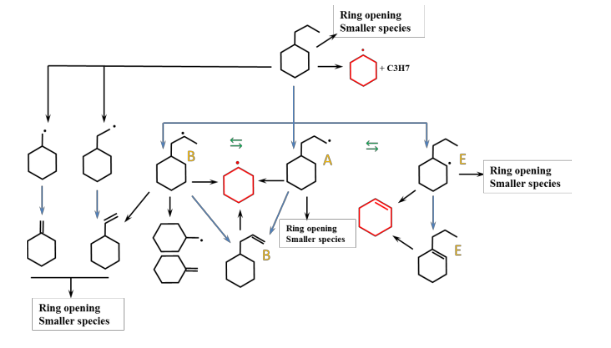
\includegraphics[scale=0.5, keepaspectratio]{images/PCH-schematic.png}
    \caption{High temperature reaction pathways of propyl-cyclohexane (PCH) as described by Abbasi et al. \cite{Abbasi2018KineticFormation}}
    \label{fig:pch-pathways}
\end{figure}


\newpage

\section{Reaction Pathways of n-propyl-cyclohexane Kinetic Model}
N-propyl-cyclohexane follows the class of reactions for its oxidation starting with a unimolecular fuel decomposition and hydrogen abstraction reactions, and further down through a series of steps. H-abstraction reactions occur at high to produce cycloalkyl radicals with different radicals sites - sites on the cyclic ring and sites on the alkyl groups. These class of reactions was proposed by Pousse et al.\cite{Pousse2010LeanN-Propylcyclohexane} in the oxidation mechanism of n-propyl-cyclohexane as a constituent of diesel fuel surrogates. 

At high temperatures, H-abstraction reactions occur via a $\beta$-scission - simply meaning that when the H-atom is removed, the radical is formed on the adjacent carbon atom to ensure thermodynamic stability. Nonetheless, since at high temperatures, there is sufficient energy and collisions occur more rapidly, the radical though stable isomerizes and forms other radicals within the cycloalkyl radical atom with molecular formula \ce{C9H17}. These radicals can also form if the ring decomposes along the \ce{C-C} bonds through $\beta$-scissions and letting go of yet another hydrogen to form a first a biradical and then a double bond - olefins (propenyl-cyclohexane or propyl-cyclohexene) with another radical species, thus having a combination of Intra\textunderscore RH\textunderscore Add\textunderscore Endocyclic reactions to produce acyclic nonene in fig.\ref{fig:nonene } and that of R\textunderscore Addition\textunderscore MultipleBond on the cycloalkyl radicals to give propenyl-cyclohexane (double bonds on the alkyl group) and propyl-cyclohexene (double bond on the ring) through $\beta$-scissions.
  
  
  \begin{figure}[!htp]
      \centering
      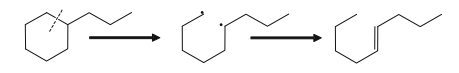
\includegraphics[keepaspectratio]{images/nonene.png}
      \caption{Unimolecular initiation of the PCH bonds forming acyclic nonene \cite{Pousse2010LeanN-Propylcyclohexane}}
      \label{fig:nonene }
  \end{figure}
  
\subsection{High Temperature mechanism of propyl-cyclohexane}
  From fig.\ref{fig:pch-pathways}, the main class of reactions that make up the dominant reaction pathways for PCH are:
  \begin{enumerate}
      \item Unimolecular fuel decomposition
      \item H-atom abstraction leading to cycloalkyl radicals
      \item $\beta$-scission decomposition along the \ce{C-C} bonds to give acyclic biradicals and eventually Olefins
      \item Dehydrogenation leading to benezene and smaller radicals 
      \item Isomerization and decomposition of radicals after the ring opening
  \end{enumerate}

The various stages of the reactions are dependent on temperature, thus at higher temperatures the chain branching is not as complex, however at lower temperature many reaction pathways are possible. Addition of \ce{O2} to the cycloalkyl radicals to form \ce{cyROO^.} also happens at high temperatures but is more dominant in the low temperature mechanism as well as the formation of hydroperoxy-cycloalkyl radicals eventually leading to cyclic ketohyroperoxide radicals. The final reaction flux pathways are shown in fig.\ref{fig:pch-pfa}.


\begin{figure}
    \centering
    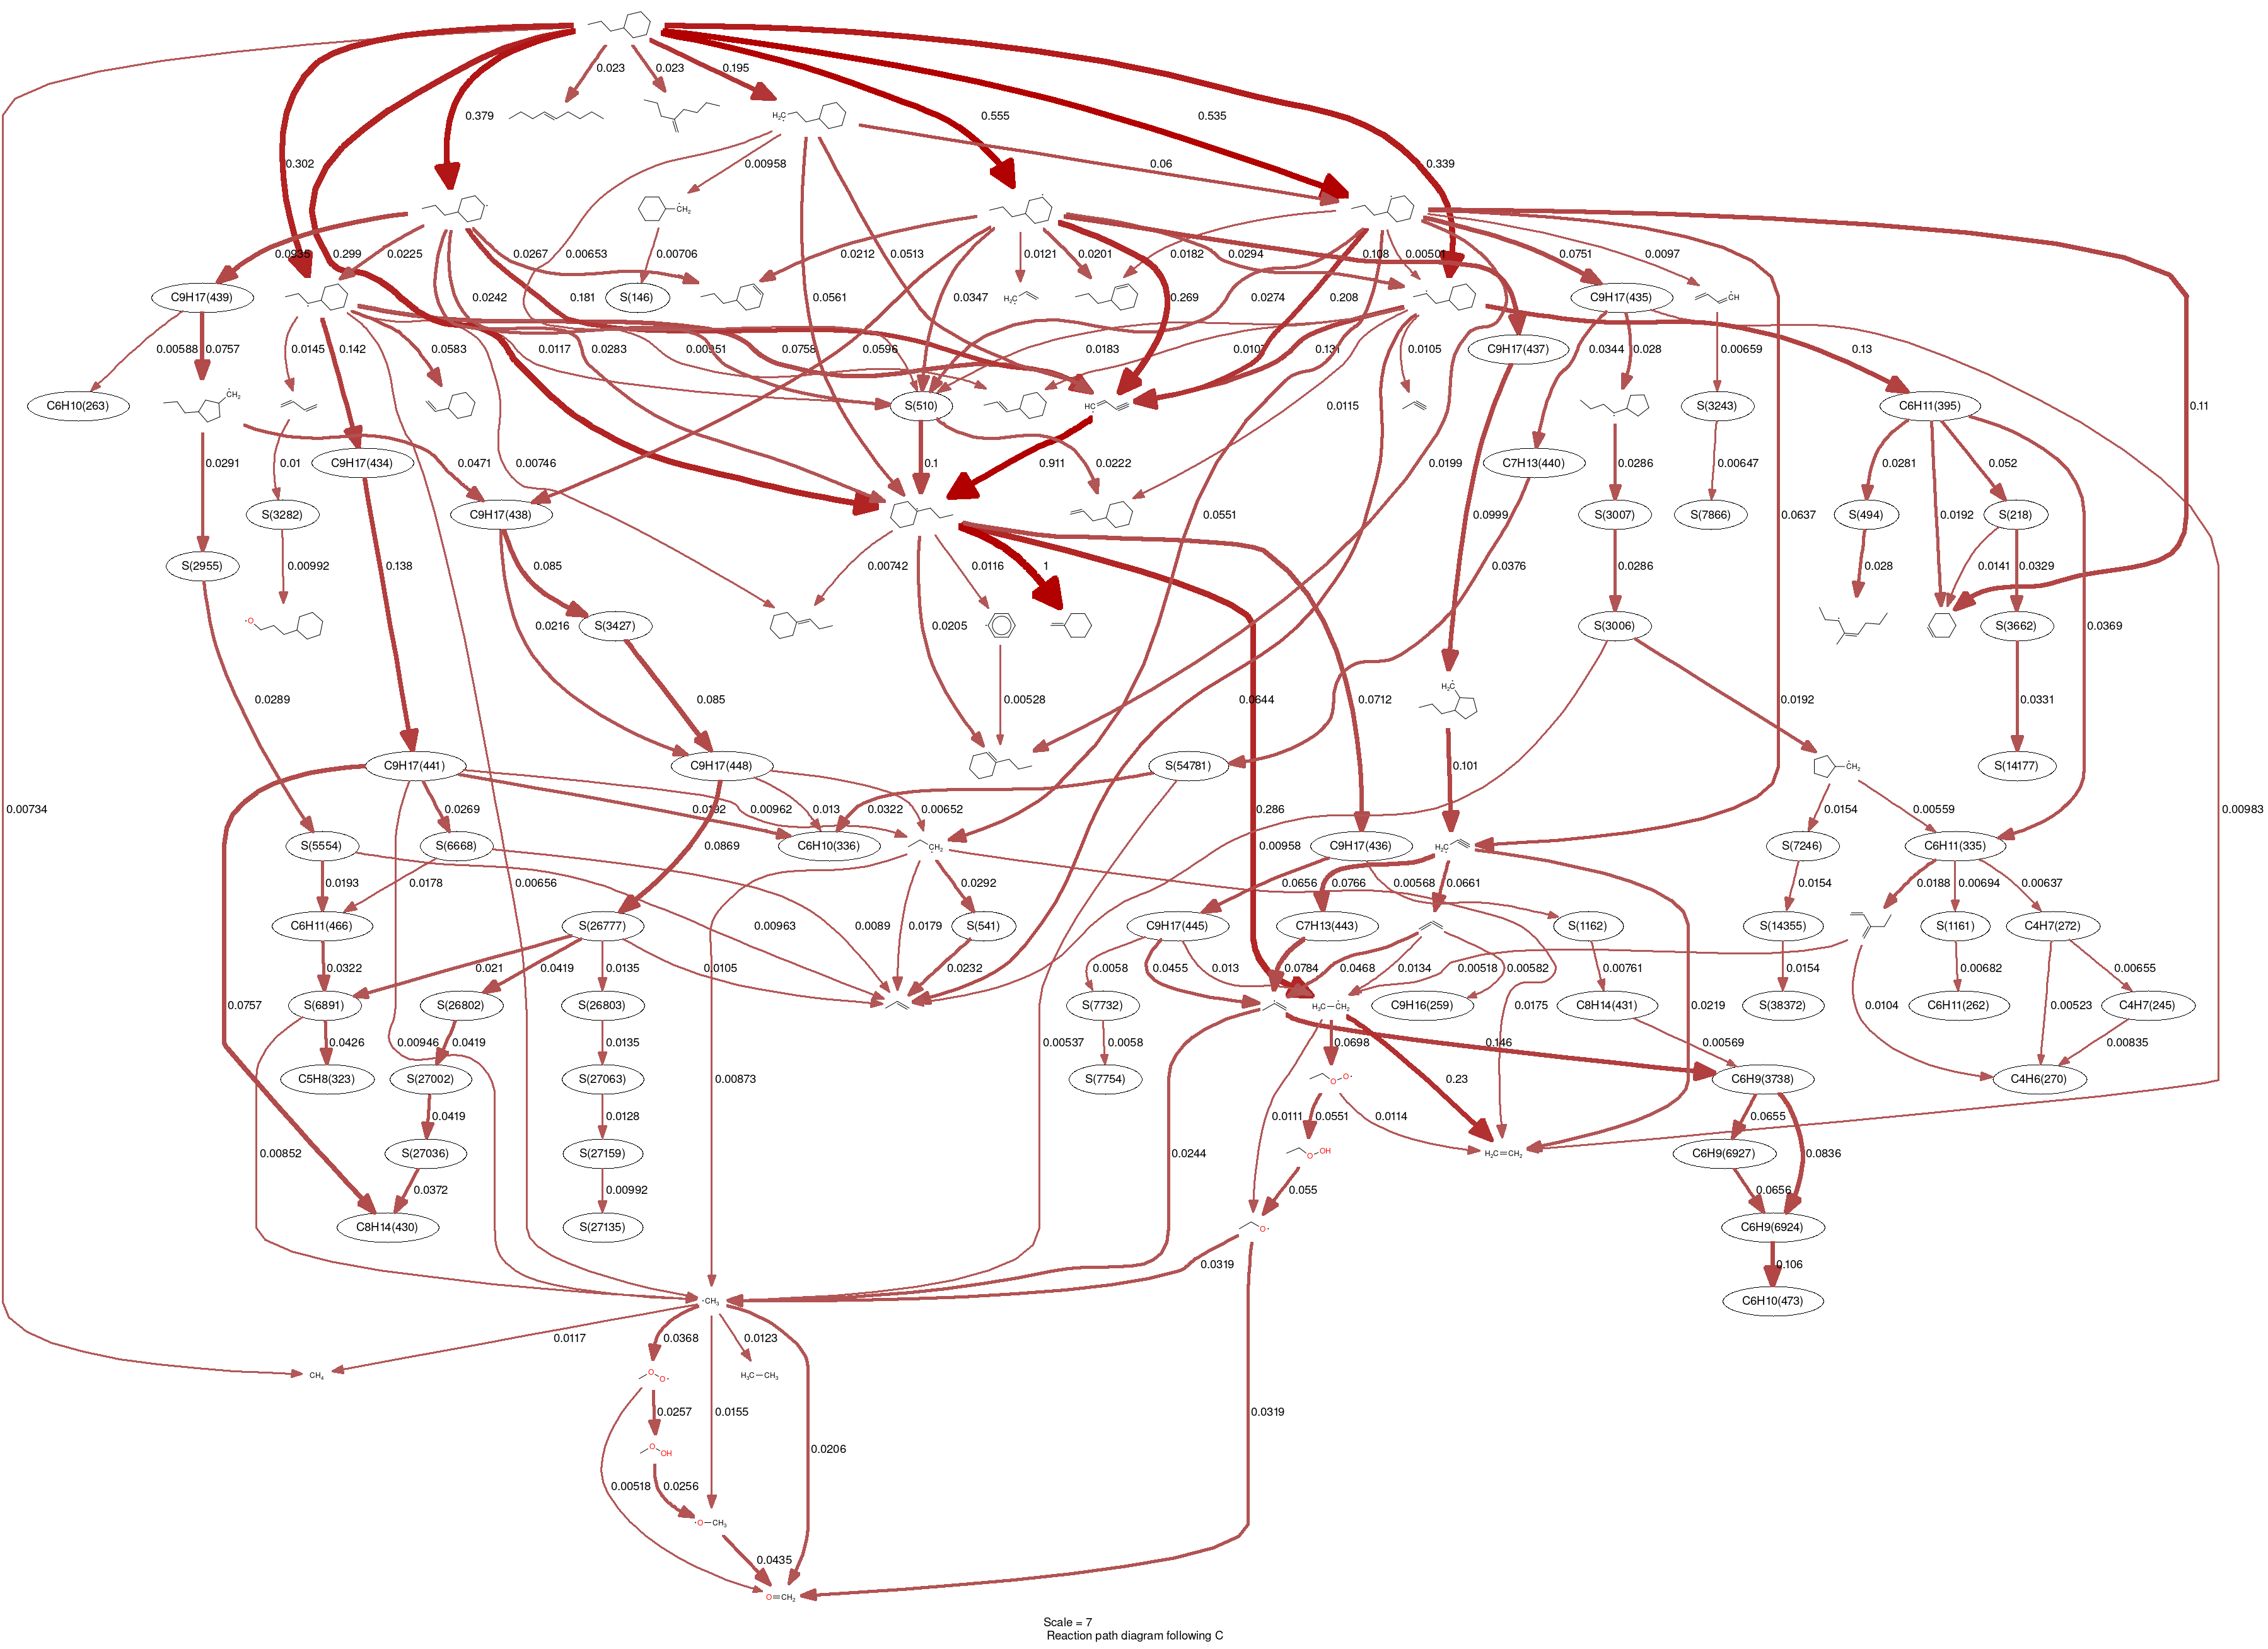
\includegraphics[scale=0.175, keepaspectratio]{images/pch-pfa.png}
    \caption{Path flux diagram of PCH model @ 1100 K and 20 atm}
    \label{fig:pch-pfa}
\end{figure}
\cleardoublepage
\subsection{Model validation of n-propyl-cyclohexane in shock tubes for ignition delay time predictions}
Shock tubes essentially devices designed to experiment and study the flow of high-temperature and high-velocity effects of compressible gases within an actual engine-like environment. It is designed on the basis of knowledge of gas dynamics and analysing shock waves. It operates on the principle that at high temperatures, supersonic gases flow is in the tube a diaphragm causes a separation into regions of high-pressure and low-pressure. As the pressure rises, an unsteady rarefied wave passes into the driver gas with a velocity usually a few kilometers per second causing flow from the high-pressure region to the low-pressure region. As the shock wave progresses in the low-pressure region, it pushes the low-pressure gas ahead of it. Thus, creating two fronts, flow ahead of the shock wave and flow behind the shock wave. The flow ahead of the behind the shock wave (driver gas) is the gas of interest. The velocity of the driver gas is equal to  that of the driven gas\cite{Greene1964TheR.}. Usually, there in the high-pressure region, is an explosive gas which is the gas studied, and present is a laser beam to detect the luminescence of some excited species. The ignition delay time can be defined as the time it takes:
\begin{enumerate}
    \item For the shock wave to hit the wall and propagate with the excitation of a \ce{CH*} or \ce{OH*}radical
    \item For the shock wave to hit the wall and measurement of the highest peak of the temperature in the driven section
    \item For the shock wave to hit the wall and detection of the highest peak of the pressure in the driven section
\end{enumerate}
Since all three possibilities of measuring the ignition delay time data in shock tubes exist, it is often well defined based on one of the three main possibilities usually for the first-stage ignition \cite{Davidson2004InterpretingData}\cite{Fieweger1994Shock-tubePressures}\cite{Fieweger1997Self-ignitionPressure}\cite{Pfahl1996Self-ignitionConditions}\cite{Haylett2012IgnitionTube}

In Cantera, this process is often defined based on the reactor type of interest. First, the gas solution object is created with the \textbf{gas.Solution} class, then a reactor type is selected with the appropriate initial conditions usually coming from the experimental data being validated against. Next, the state of the system is set with the reactor network previously defined and then a simulation in time for the next states is found using the ODE solver. The ODE solver starts at the current state  of the systems and progresses in time by one of the following methods:
\begin{enumerate}
    \item \textbf{step()}: This involves a reactor step from the current state of the system by solving the previous state of the system using the time step given. This is an explicit method where the ODE solver internally solves the numerical Differential Algebraic Equations (DAE) system. The new time is returned as well as the state of the system at the next state using the previously defined time step $\Delta$t within the solver absolute and relative tolerances. The time step cannot be larger than the maximum time step or else the ODE solver breaks.
    \item \textbf{advance($t_{new}$)}: This method solves the state of the system at a predefined step times $t_{new}$. This $t_{new}$ describes the absolute time of the system from the initial system by calling the ignition delay time function for the reactor in a loop, either a while loop or for loop at exactly the time specified - basically using the \textbf{step():} function several times in the process. In addition, the \textbf{advance():} function can be made to continue until a steady-state solution is attained by time stepping. Only when the feature-scaled residual of the state vector is below a given threshold value is the system at steady-state and the ODE solver stops.
\end{enumerate} 
For all shock tube models in this work, a zero-dimensional homogeneous closed ideal gas reactor with constant volume and internal energy class was used since at constant volume, there is no P-V work done against the control volume of the gas. Since the temperature is known, the energy equation is computed assuming adiabatic conditions in the reactor volume. The time integration of the species is computed in uniform time steps until the solution is found. During the time integration, the reactor model scheme usually an ODE SUNDIALS solver \cite{hindmarsh2005sundials} solves the differential equations of the species within the energy equation. The energy equation accounts for the energy interaction via the heat equation but is ignored since the reactor assumes adiabatic conditions and indicates only mechanical work interactions, mass transport due to species diffusion and conversion.  The equation being solved in the ideal gas reactor  of Cantera is equation \ref{eq.mass conservation} as given by Robert Kee et al's book on Chemically Reacting Flow \cite{Kee2003ChemicallyPractice}. The definition of the ignition delay time varies. Nonetheless, the model used in Cantera assumes an ignition delay time based on the excited \ce{CH} or \ce{OH} radical species and is often very close to the highest temperature spike Ji et al point out for the sensitivity analysis of ignition delay times \cite{Ji2019EvolutionAutoignition}. 

\begin{equation}
    U = m\sum_k{Y_k u_k(T)}
\end{equation}

\begin{equation}
    \frac{dU}{dt} = u\frac{dm}{dt}+mc_v\frac{dT}{dt}+m\sum_k{u_k \frac{dY_k}{dt}}
\end{equation}

\[\text{Substituting the corresponding derivations for temperature in the reactor as:} \]


\begin{equation}
    mc_v\frac{dT}{dt}=-p\frac{dV}{dt} - Q^. + \sum_{in}{m_{in}(h_{in}- \sum_k{u_k Y_{k, in}}) -\frac{pV}{m}\sum_{out}{m_{out}^.} - \sum_k{m_{k, gen}^. u_k}}
    \label{eq.mass conservation}
\end{equation}

The ignition delay times prediction are presented as modeled in Cantera against shock tube experiments of Dubois et al.\cite{Dubois2009ExperimentalConditions} and Tian et al. \cite{Tian2014ComparativeN-Propylcyclohexane} .

As seen in fig. \ref{fig:pch-idt-dubois}, there is close agreement at to experiments of Dubois et al.\cite{Dubois2009ExperimentalConditions} who studied n-prpylcyclohexane under engine-like conditions in a shock tube and spherical bomb using the chemiluminescence of \ce{OH^*} and \ce{CH^*}radicals for the ignition delay of PCH \ \ce{O2} \ \ce{Ar} mixtures for $\phi=0.2$, $\phi=0.3$, $\phi=0.4$ and $\phi=0.5$ at 10 bar. As the model progresses further, there is more deviation between the model prediction of ignition delay times against the experiments of Tian et al. who studied the ignition delay times of several cyclohexane fuels - cyclohexane, ethylcyclohexane and n-propylcyclohexane at atmospheric pressure between lean, stoichiometric and rich fuel mixtures. The prediction at $\phi=2.0$ is unpredicted and a sensitivity analysis would be helpful to understand which reactions control the ignition delay time predictions.


\begin{figure}[!hbp]
    \centering
    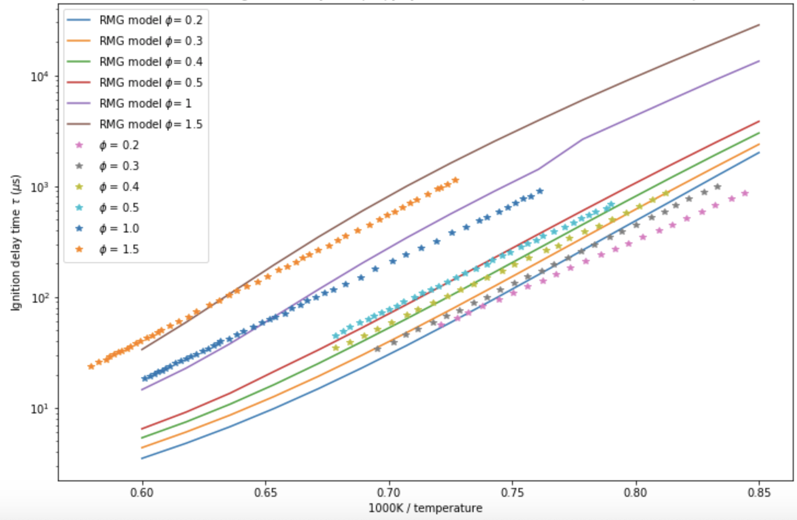
\includegraphics[scale=0.4, keepaspectratio]{images/pch-idt-dubois.png}
    \caption{Ignition delay time prediction of propyl-cyclohexane/air at 10 bar for $\phi=0.2$,$\phi=0.3$,$\phi=0.4$, $\phi=0.5$, $\phi=1.0$ and $\phi=1.5$ against experiments of Dubois et al. \cite{Dubois2009ExperimentalConditions}. Lines indicate model predictions and symbols indicate experiments}
    \label{fig:pch-idt-dubois}
\end{figure}



\begin{figure}[!htp]
    \centering
    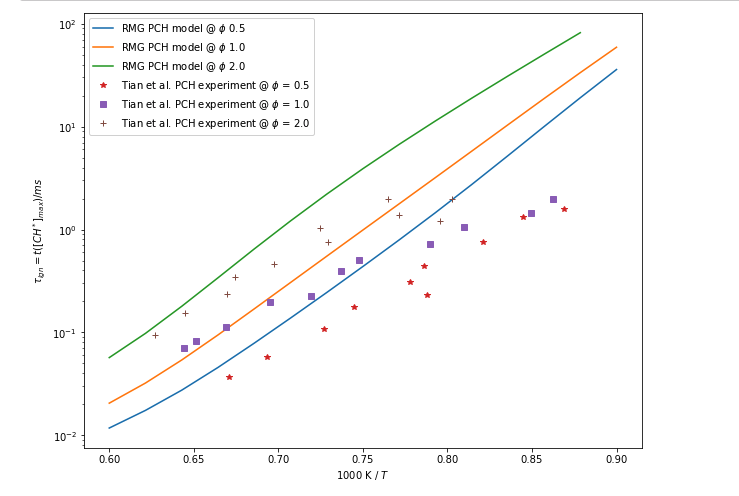
\includegraphics[scale=0.4, keepaspectratio]{images/pch-model-idt.png}
    \caption{Ignition delay time prediction of propyl-cyclohexane/air at 1 atm for $\phi=0.5$, $\phi=1.0$ and $\phi=2.0$ against experiments of Tian et al. \cite{Tian2014ComparativeN-Propylcyclohexane}. Lines indicate model predictions and symbols indicate experiments}
    \label{fig:pch-idt}
\end{figure}


\subsubsection{Sensitivity Analysis of the Ignition delay times}
A detailed analysis was done to determine which control variables control the ignition delay of the iso-octane model. Since the species usually measured for the onset of ignition is the \ce{OH^.} radical \cite{Ji2019EvolutionAutoignition}, the concentration of the \ce{OH^.} radical was used as the criteria for sensitivity by the use of a brute force method comparing the localised sensitivity at a given temperature for all the top 10 most sensitive reactions that influence the ignition delay time. This sensitivity analysis was done at high temperatures of 1250 K to observe which reactions contribute the most to either the production or consumption of the \ce{OH^.} radical species. 

The sensitivity analysis involves the perturbation of both the forward and reverse rates of the 20 most sensitive reactions to \ce{OH^.} radical concentration by a factor of two and then comparing the change in the ignition delay time to the preset (original )rate constant of those same reaction ignition delay time sensitivity coefficients to the \ce{OH^.} radical species. The magnitude of the sensitivity coefficient indicates a strong dependence on \ce{OH^.} radical concentration, while the sign indicates rate of production if positive and rate of consumption if negative. The sensitivity plots are shown in fig.\ref{fig:pch-sensitivity}.

The summary of the RMG n-propyl-cyclohexane model is given in table \ref{tab:pch_model_summary}. 
\begin{table}[ht]
\arrayrulecolor[HTML]{DB5800}
\caption{Summary of RMG n-propyl-cyclohexane model analysis and Ignition delay time prediction at extinction }
\centering
\begin{adjustbox}{width=1\textwidth}
\begin{tabular}{ p{6cm} c c c c }
\rowcolor{lightgray}\multicolumn{4}{|c|}{RMG n-propyl-cyclohexane model summary} \\
Number of Species before model generation stopped & 682 & &  \\ 
Number of species after model generation stopped  & 851 & &  \\
Number of Reactions before model generation stopped & 29174 & & \\ 
Number of reactions after model generation stopped & 49638 & & \\ 
\hline
 Model ignition delay time at extinction &  Temperature & Pressure & Equivalence ratio \\
 \begin{tabular}{ c }
    $\tau$=35.8521 ms   \\
    $\tau$=59.0368 ms \\ 
    $\tau$=81.7375 ms \\
 \end{tabular} & \begin{tabular}{ c } 
       1111.11 K\\
      1111.11 K \\
      1111.11 K \\
 \end{tabular} & 1 atm & \begin{tabular}{ c }
      $\phi=0.5$  \\
      $\phi=1.0$ \\
      $\phi=2.0$ \\
 \end{tabular} \\
 \end{tabular}
    \end{adjustbox}
    \label{tab:pch_model_summary}
\end{table}


\begin{figure}
    \centering
    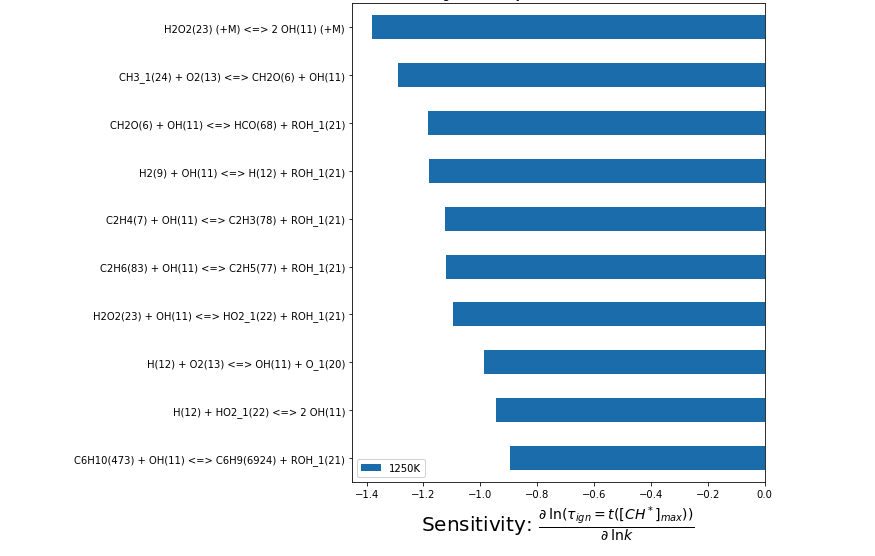
\includegraphics[scale=0.45, keepaspectratio]{images/pch-sensitivity.png}
    \caption{Sensitivity coefficients of the ignition delay time of the n-propyl-cyclohexane model to \ce{OH^.} radical concentration at stoichiometric fuel/air mixture at 1250 K at $P=1$ atm. Where the ignition delay times $\tau_{ign}=t(\ce{CH^.}_{max})$}
    \label{fig:pch-sensitivity}
\end{figure}

